\documentclass[12pt,a4paper,openany]{book}
\usepackage{lmodern}
\usepackage[svgnames]{xcolor} % Required to specify font color
\usepackage{xcolor}
\definecolor{vert1}{rgb}{0.0,0.3.9,0.0}
\definecolor{bleu}{rgb}{0,0,0.5}
\definecolor{bleu3}{rgb}{1,0.2,0.2}
\definecolor{grisgris}{gray}{0.4}
\definecolor{grisclair}{HTML}{E7E7E7}
\definecolor{grisfonce}{HTML}{A5A5A5}
\definecolor{rougeUPS}{rgb}{0.6, 0.3, 0.3}

\fboxsep =0pt \parindent =0pt\parskip =12pt



\usepackage[utf8]{inputenc} 
\usepackage[T1]{fontenc}
\usepackage[francais]{babel}
\usepackage[top=1.7cm, bottom=1.7cm, left=1.7cm, right=1.7cm]{geometry}
\usepackage{verbatim}
\usepackage[urlbordercolor={1 1 1}, linkbordercolor={1 1 1}, linkcolor=vert1, urlcolor=bleu, colorlinks=true]{hyperref}
\usepackage{tikz} %Vectoriel
\usepackage{listings}
\usepackage{fancyhdr}
\usepackage{multido}
\usepackage{amssymb}
\usepackage{float}
\usepackage[francais]{minitoc}
\usepackage[final]{pdfpages} 
\usepackage{graphicx} % Required for box manipulation

\newcommand{\titre}{Base de données}
\newcommand{\subtitle}{SQL}
\newcommand{\auteur}{Antoine de \bsc{Roquemaurel}}
\newcommand{\formation}{L3 Informatique}
\newcommand{\semestre}{5}
\newcommand{\annee}{2013}
\newcommand{\prof}{~}


\newcommand{\pole}{}
\newcommand{\sigle}{bdd}


\definecolor{gris1}{gray}{0.40}
\definecolor{gris2}{gray}{0.55}
\definecolor{gris3}{gray}{0.65}
\definecolor{gris4}{gray}{0.50}
\definecolor{vert}{rgb}{0,0.4,0}
\definecolor{violet}{rgb}{0.65, 0.2, 0.65}
\definecolor{bleu1}{rgb}{0,0,0.8}
\definecolor{bleu2}{rgb}{0,0.2,0.6}
\definecolor{bleu3}{rgb}{0,0.2,0.2}
\definecolor{rouge}{HTML}{F93928}


\lstdefinelanguage{algo}{%
   morekeywords={%
    %%% couleur 1
		importer, programme, glossaire, fonction, procedure, constante, type, 
	%%% IMPORT & Co.
		si, sinon, alors, fin, tantque, debut, faire, lorsque, fin lorsque, 
		declenche, declencher, enregistrement, tableau, retourne, retourner, =, pour, a,
		/=, <, >, traite,exception, 
	%%% types 
		Entier, Reel, Booleen, Caractere, Réél, Booléen, Caractère,
	%%% types 
		entree, maj, sortie,entrée,
	%%% types 
		et, ou, non,
	},
  sensitive=true,
  morecomment=[l]{--},
  morestring=[b]',
}

\lstset{language=algo,
    %%% BOUCLE, TEST & Co.
      emph={importer, programme, glossaire, fonction, procedure, constante, type},
      emphstyle=\color{bleu2},
    %%% IMPORT & Co.  
	emph={[2]
		si, sinon, alors, fin , tantque, debut, faire, lorsque, fin lorsque, 
		declencher, retourner, et, ou, non,enregistrement, retourner, retourne, 
		tableau, /=, <, =, >, traite,exception, pour, a
	},
      emphstyle=[2]\color{bleu1},
    %%% FONCTIONS NUMERIQUES
      emph={[3]Entier, Reel, Booleen, Caractere, Booléen, Réél, Caractère},
      emphstyle=[3]\color{gris1},
    %%% FONCTIONS NUMERIQUES
      emph={[4]entree, maj, sortie, entrée},	
      emphstyle=[4]\color{gris1},
}
\lstdefinelanguage{wl}{%
   morekeywords={%
    %%% couleur 1
		importer, programme, glossaire, fonction, procedure, constante, type, 
	%%% IMPORT & Co.
		si, sinon, alors, fin, TANTQUE, tantque, FIN, PROCEDURE, debut, faire, lorsque, 
		fin lorsque, declenche, declencher, enregistrement, tableau, retourne, retourner, =, 
		/=, <, >, traite,exception, 
	%%% types 
		Entier, Reel, Booleen, Caractere, Réél, Booléen, Caractère,
	%%% types 
		entree, maj, sortie,entrée,
	%%% types 
		et, ou, non,
	},
  sensitive=true,
  morecomment=[l]{//},
  morestring=[b]',
}

\lstset{language=wl,
    %%% BOUCLE, TEST & Co.
      emph={importer, programme, glossaire, fonction, procedure, constante, type},
      emphstyle=\color{bleu2},
    %%% IMPORT & Co.  
	emph={[2]
		si, sinon, alors, fin , tantque, debut, faire, lorsque, fin lorsque, 
		declencher, retourner, et, ou, non,enregistrement, retourner, retourne, 
		tableau, /=, <, =, >, traite,exception
	},
      emphstyle=[2]\color{bleu1},
    %%% FONCTIONS NUMERIQUES
      emph={[3]Entier, Reel, Booleen, Caractere, Booléen, Réél, Caractère},
      emphstyle=[3]\color{gris1},
    %%% FONCTIONS NUMERIQUES
      emph={[4]entree, maj, sortie, entrée},	
      emphstyle=[4]\color{gris1},
}
\lstdefinelanguage{css}{%
   morekeywords={%
    %%% couleur 1
		background, image, repeat, position, index, color, border, font, 
		size, url, family, style, variant, weight, letter, spacing, line, 
		height, text, decoration, align, indent, transform, shadow, 
		background, image, repeat, position, index, color, border, font, 
		size, url, family, style, variant, weight, letter, spacing, line, 
		height, text, decoration, align, indent, transform, shadow, 
		vertical, align, white, space, word, spacing,attachment, width, 
		max, min, margin, padding, clip, direction, display, overflow,
		visibility, clear, float, top, right, bottom, left, list, type, 
		collapse, side, empty, cells, table, layout, cursor, marks, page, break,
		before, after, inside, orphans, windows, azimuth, after, before, cue, 
		elevation, pause, play, during, pitch, range, richness, spek, header, 
		numeral, punctuation, rate, stress, voice, volume,
	%%% types 
		left, right, bottom, top, none, center, solid, black, blue, red, green,
	},
  sensitive=true,
  sensitive=true,
  morecomment=[s]{/*}{*/},
  morestring=[b]',
}
\lstset{language=css,
    %%% BOUCLE, TEST & Co.
      emph={
		background, image, repeat, position, index, color, border, font, 
		size, url, family, style, variant, weight, letter, spacing, line, 
		height, text, decoration, align, indent, transform, shadow, 
		background, image, repeat, position, index, color, border, font, 
		size, url, family, style, variant, weight, letter, spacing, line, 
		height, text, decoration, align, indent, transform, shadow, 
		vertical, align, white, space, word, spacing,attachment, width, 
		max, min, margin, padding, clip, direction, display, overflow,
		visibility, clear, float, top, right, bottom, left, list, type, 
		collapse, side, empty, cells, table, layout, cursor, marks, page, break,
		before, after, inside, orphans, windows, azimuth, after, before, cue, 
		elevation, pause, play, during, pitch, range, richness, spek, header, 
		numeral, punctuation, rate, stress, voice, volume,
	  },
      emphstyle=\color{bleu2},
    %%% FONCTIONS NUMERIQUES
      emph={[3]
		left, right, bottom, top,none, solid, black, blue, green,
		  },
      emphstyle=[3]\color{bleu3},
    %%% FONCTIONS NUMERIQUES
}

\lstset{language=SQL,
    %%% BOUCLE, TEST & Co.
      emph={INSERT, UPDATE, DELETE, WHERE, SET, GROUP, BY, ORDER, REFERENCES},
      emphstyle=\color{bleu2},
    %%% IMPORT & Co.  
	emph={[2]
		if, end, begin, then, for, each, else, after, of, on, to
	},
      emphstyle=[2]\color{bleu1},
    %%% FONCTIONS NUMERIQUES
      emph={[3]Entier, Reel, Booleen, Caractere, Booléen, Réél, Caractère},
      emphstyle=[3]\color{gris1},
    %%% FONCTIONS NUMERIQUES
      emph={[4]entree, maj, sortie, entrée},	
      emphstyle=[4]\color{gris1},
}
\lstdefinelanguage{ARM}{%
   morekeywords={%
   ADD, SUB, MOV, MUL, RSB,CMP, BLS, BLE, B,BHI,LDR,
   BGE, RSBLT, BGT, BEQ, BNE,BLT,BHS,STR,STRB
	},
  sensitive=true,
  morecomment=[l]{@},
  morestring=[b]',
}

\lstset{ % general style for listings 
   numbers=left 
   , literate={é}{{\'e}}1 {è}{{\`e}}1 {à}{{\`a}}1 {ê}{{\^e}}1 {É}{{\'E}}1 {ô}{{\^o}}1 {€}{{\euro}}1{°}{{$^{\circ}$}}1 {ç}{ {c}}1 {ù}{u}1
	, extendedchars=\true
   , tabsize=2 
   , frame=l
   , framerule=1.1pt
   , linewidth=520px
   , breaklines=true 
   , basicstyle=\footnotesize\ttfamily 
   , numberstyle=\tiny\ttfamily 
   , framexleftmargin=0mm 
   , xleftmargin=0mm 
   , captionpos=b 
	, keywordstyle=\color{bleu2}
	, commentstyle=\color{vert}
	, stringstyle=\color{rouge}
	, showstringspaces=false
	, extendedchars=true
	, mathescape=true
} 
%	\lstlistoflistings
%	\addcontentsline{toc}{part}{List of code examples}

\documentclass[12pt,a4paper,openany]{book}
\usepackage{lmodern}
\usepackage{xcolor}
\usepackage{xcolor}
\definecolor{vert1}{rgb}{0.0,0.3.9,0.0}
\definecolor{bleu}{rgb}{0,0,0.5}
\definecolor{bleu3}{rgb}{1,0.2,0.2}
\definecolor{grisgris}{gray}{0.4}
\definecolor{grisclair}{HTML}{E7E7E7}
\definecolor{grisfonce}{HTML}{A5A5A5}
\definecolor{rougeUPS}{rgb}{0.6, 0.3, 0.3}

\fboxsep =0pt \parindent =0pt\parskip =12pt



\usepackage[utf8]{inputenc}
\usepackage[T1]{fontenc}
\usepackage[francais]{babel}
\usepackage[top=1.7cm, bottom=1.7cm, left=1.7cm, right=1.7cm]{geometry}
\usepackage{verbatim}
\usepackage[urlbordercolor={1 1 1}, linkbordercolor={1 1 1}, linkcolor=vert1, urlcolor=bleu, colorlinks=true]{hyperref}
\usepackage{tikz} %Vectoriel
\usepackage{listings}
\usepackage{fancyhdr}
\usepackage{multido}
\usepackage{amssymb}
\usepackage{float}

\newcommand{\titre}{Complexité des algorithmes}

\newcommand{\pole}{}
\newcommand{\sigle}{complexite}

\newcommand{\semestre}{3}

\definecolor{gris1}{gray}{0.40}
\definecolor{gris2}{gray}{0.55}
\definecolor{gris3}{gray}{0.65}
\definecolor{gris4}{gray}{0.50}
\definecolor{vert}{rgb}{0,0.4,0}
\definecolor{violet}{rgb}{0.65, 0.2, 0.65}
\definecolor{bleu1}{rgb}{0,0,0.8}
\definecolor{bleu2}{rgb}{0,0.2,0.6}
\definecolor{bleu3}{rgb}{0,0.2,0.2}
\definecolor{rouge}{HTML}{F93928}


\lstdefinelanguage{algo}{%
   morekeywords={%
    %%% couleur 1
		importer, programme, glossaire, fonction, procedure, constante, type, 
	%%% IMPORT & Co.
		si, sinon, alors, fin, tantque, debut, faire, lorsque, fin lorsque, 
		declenche, declencher, enregistrement, tableau, retourne, retourner, =, pour, a,
		/=, <, >, traite,exception, 
	%%% types 
		Entier, Reel, Booleen, Caractere, Réél, Booléen, Caractère,
	%%% types 
		entree, maj, sortie,entrée,
	%%% types 
		et, ou, non,
	},
  sensitive=true,
  morecomment=[l]{--},
  morestring=[b]',
}

\lstset{language=algo,
    %%% BOUCLE, TEST & Co.
      emph={importer, programme, glossaire, fonction, procedure, constante, type},
      emphstyle=\color{bleu2},
    %%% IMPORT & Co.  
	emph={[2]
		si, sinon, alors, fin , tantque, debut, faire, lorsque, fin lorsque, 
		declencher, retourner, et, ou, non,enregistrement, retourner, retourne, 
		tableau, /=, <, =, >, traite,exception, pour, a
	},
      emphstyle=[2]\color{bleu1},
    %%% FONCTIONS NUMERIQUES
      emph={[3]Entier, Reel, Booleen, Caractere, Booléen, Réél, Caractère},
      emphstyle=[3]\color{gris1},
    %%% FONCTIONS NUMERIQUES
      emph={[4]entree, maj, sortie, entrée},	
      emphstyle=[4]\color{gris1},
}
\lstdefinelanguage{wl}{%
   morekeywords={%
    %%% couleur 1
		importer, programme, glossaire, fonction, procedure, constante, type, 
	%%% IMPORT & Co.
		si, sinon, alors, fin, TANTQUE, tantque, FIN, PROCEDURE, debut, faire, lorsque, 
		fin lorsque, declenche, declencher, enregistrement, tableau, retourne, retourner, =, 
		/=, <, >, traite,exception, 
	%%% types 
		Entier, Reel, Booleen, Caractere, Réél, Booléen, Caractère,
	%%% types 
		entree, maj, sortie,entrée,
	%%% types 
		et, ou, non,
	},
  sensitive=true,
  morecomment=[l]{//},
  morestring=[b]',
}

\lstset{language=wl,
    %%% BOUCLE, TEST & Co.
      emph={importer, programme, glossaire, fonction, procedure, constante, type},
      emphstyle=\color{bleu2},
    %%% IMPORT & Co.  
	emph={[2]
		si, sinon, alors, fin , tantque, debut, faire, lorsque, fin lorsque, 
		declencher, retourner, et, ou, non,enregistrement, retourner, retourne, 
		tableau, /=, <, =, >, traite,exception
	},
      emphstyle=[2]\color{bleu1},
    %%% FONCTIONS NUMERIQUES
      emph={[3]Entier, Reel, Booleen, Caractere, Booléen, Réél, Caractère},
      emphstyle=[3]\color{gris1},
    %%% FONCTIONS NUMERIQUES
      emph={[4]entree, maj, sortie, entrée},	
      emphstyle=[4]\color{gris1},
}
\lstdefinelanguage{css}{%
   morekeywords={%
    %%% couleur 1
		background, image, repeat, position, index, color, border, font, 
		size, url, family, style, variant, weight, letter, spacing, line, 
		height, text, decoration, align, indent, transform, shadow, 
		background, image, repeat, position, index, color, border, font, 
		size, url, family, style, variant, weight, letter, spacing, line, 
		height, text, decoration, align, indent, transform, shadow, 
		vertical, align, white, space, word, spacing,attachment, width, 
		max, min, margin, padding, clip, direction, display, overflow,
		visibility, clear, float, top, right, bottom, left, list, type, 
		collapse, side, empty, cells, table, layout, cursor, marks, page, break,
		before, after, inside, orphans, windows, azimuth, after, before, cue, 
		elevation, pause, play, during, pitch, range, richness, spek, header, 
		numeral, punctuation, rate, stress, voice, volume,
	%%% types 
		left, right, bottom, top, none, center, solid, black, blue, red, green,
	},
  sensitive=true,
  sensitive=true,
  morecomment=[s]{/*}{*/},
  morestring=[b]',
}
\lstset{language=css,
    %%% BOUCLE, TEST & Co.
      emph={
		background, image, repeat, position, index, color, border, font, 
		size, url, family, style, variant, weight, letter, spacing, line, 
		height, text, decoration, align, indent, transform, shadow, 
		background, image, repeat, position, index, color, border, font, 
		size, url, family, style, variant, weight, letter, spacing, line, 
		height, text, decoration, align, indent, transform, shadow, 
		vertical, align, white, space, word, spacing,attachment, width, 
		max, min, margin, padding, clip, direction, display, overflow,
		visibility, clear, float, top, right, bottom, left, list, type, 
		collapse, side, empty, cells, table, layout, cursor, marks, page, break,
		before, after, inside, orphans, windows, azimuth, after, before, cue, 
		elevation, pause, play, during, pitch, range, richness, spek, header, 
		numeral, punctuation, rate, stress, voice, volume,
	  },
      emphstyle=\color{bleu2},
    %%% FONCTIONS NUMERIQUES
      emph={[3]
		left, right, bottom, top,none, solid, black, blue, green,
		  },
      emphstyle=[3]\color{bleu3},
    %%% FONCTIONS NUMERIQUES
}

\lstset{language=SQL,
    %%% BOUCLE, TEST & Co.
      emph={INSERT, UPDATE, DELETE, WHERE, SET, GROUP, BY, ORDER, REFERENCES},
      emphstyle=\color{bleu2},
    %%% IMPORT & Co.  
	emph={[2]
		if, end, begin, then, for, each, else, after, of, on, to
	},
      emphstyle=[2]\color{bleu1},
    %%% FONCTIONS NUMERIQUES
      emph={[3]Entier, Reel, Booleen, Caractere, Booléen, Réél, Caractère},
      emphstyle=[3]\color{gris1},
    %%% FONCTIONS NUMERIQUES
      emph={[4]entree, maj, sortie, entrée},	
      emphstyle=[4]\color{gris1},
}
\lstdefinelanguage{ARM}{%
   morekeywords={%
   ADD, SUB, MOV, MUL, RSB,CMP, BLS, BLE, B,BHI,LDR,
   BGE, RSBLT, BGT, BEQ, BNE,BLT,BHS,STR,STRB
	},
  sensitive=true,
  morecomment=[l]{@},
  morestring=[b]',
}

\lstset{ % general style for listings 
   numbers=left 
   , literate={é}{{\'e}}1 {è}{{\`e}}1 {à}{{\`a}}1 {ê}{{\^e}}1 {É}{{\'E}}1 {ô}{{\^o}}1 {€}{{\euro}}1{°}{{$^{\circ}$}}1 {ç}{ {c}}1 {ù}{u}1
	, extendedchars=\true
   , tabsize=2 
   , frame=l
   , framerule=1.1pt
   , linewidth=520px
   , breaklines=true 
   , basicstyle=\footnotesize\ttfamily 
   , numberstyle=\tiny\ttfamily 
   , framexleftmargin=0mm 
   , xleftmargin=0mm 
   , captionpos=b 
	, keywordstyle=\color{bleu2}
	, commentstyle=\color{vert}
	, stringstyle=\color{rouge}
	, showstringspaces=false
	, extendedchars=true
	, mathescape=true
} 
%	\lstlistoflistings
%	\addcontentsline{toc}{part}{List of code examples}
 %prise en charge du langage C 
\date{\today}

\makeindex
\lfoot{Université Toulouse III -- Paul Sabatier}
\rfoot{\sigle\semestre}
%\rfoot{}
\cfoot{}
\makeglossary
\makeatletter
\def\clap#1{\hbox to 0pt{\hss #1\hss}}%
\def\ligne#1{%
\hbox to \hsize{%
\vbox{\centering #1}}}%
\def\haut#1#2#3{%
\hbox to \hsize{%
\rlap{\vtop{\raggedright #1}}%
\hss
\clap{\vtop{\centering #2}}%
\hss
\llap{\vtop{\raggedleft #3}}}}%
\def\bas#1#2#3{%
\hbox to \hsize{%
\rlap{\vbox{\raggedright #1}}%
\hss \clap{\vbox{\centering #2}}%
\hss
\llap{\vbox{\raggedleft #3}}}}%
\def\maketitle{%
\thispagestyle{empty}\vbox to \vsize{%
\haut{}{\@blurb}{}

\vfill
\vspace{1cm}
\begin{flushleft}
\usefont{OT1}{ptm}{m}{n}
\huge \@title
\end{flushleft}
\par
\hrule height 4pt
\par
\begin{flushright}
\usefont{OT1}{phv}{m}{n}
\Large \@author
\par
\end{flushright}
\vspace{1cm}
\vfill
\vfill
\bas{}{\@location, le \@date}{}
}%
\cleardoublepage
}
\def\date#1{\def\@date{#1}}
\def\author#1{\def\@author{#1}}
\def\title#1{\def\@title{#1}}
\def\location#1{\def\@location{#1}}
\def\blurb#1{\def\@blurb{#1}}
\date{\today}
\author{}
\title{}
\location{Amiens}\blurb{}
\makeatother
\title{\titre}
\author{Semestre \semestre}

\location{Toulouse}
\blurb{%
Université Toulouse III -- Paul sabatier\\
L2 Informatique\\
}%



%\title{Cours \\ \titre}
%\date{\today\\ Semestre \semestre}

%\lhead{Cours: \titre}
%\chead{}
%\rhead{\thepage}

%\lfoot{Université Paul Sabatier Toulouse III}
%\cfoot{\thepage}
%\rfoot{\sigle\semestre}

\pagestyle{fancy}
\renewcommand{\chaptermark}[1]{\markboth{\bsc{\chaptername~\thechapter{} :} #1}{}}
\renewcommand{\sectionmark}[1]{\markright{\thesection{ #1}}}
\renewcommand{\headrulewidth}{0.3pt}
\renewcommand{\footrulewidth}{0.3pt}

\fancyhf{}
\fancyhead[LE]{\leftmark}
\fancyhead[RO]{\rightmark}
\fancyfoot[LE,RO]{--~\thepage~--}
\fancyfoot[LO]{\titre{}~~---~~\sigle{}\semestre{}}
\fancyfoot[RE]{Antoine de \bsc{Roquemaurel}}

%% Cas des premières pages de chapitre
\fancypagestyle{plain}{%
	\fancyhf{}%
	\fancyfoot[L]{\titre{}~~---~~\sigle{}\semestre{}}
	\fancyfoot[R]{--~\thepage~--}
	\renewcommand{\headrulewidth}{0pt}
	\renewcommand{\footrulewidth}{0.3pt}
}
\makeatletter
\renewcommand*{\lstlistlistingname}{Liste des codes sources}
\renewcommand\listoffigures{%
    \chapter{\listfigurename}%
      \@mkboth{\MakeUppercase\listfigurename}%
              {\MakeUppercase\listfigurename}%
       \@starttoc{lof}%
    }
    \renewcommand\listoftables{%
    \chapter{\listtablename}%
    \@mkboth{\MakeUppercase{\listtablename}}%
            {\MakeUppercase{\listtablename}}%
    \@starttoc{lot}
    }

    \renewcommand\lstlistoflistings{%
    \begingroup
    \chapter{\lstlistlistingname}%
    \parskip\z@\parindent\z@\parfillskip \z@ \@plus 1fil%
    \@starttoc{lol}%
    \endgroup
    }
	\makeatother

\newcommand{\remarque}[1]{
	\begin{center}
	\medskip
	\colorbox{remarque}{
		\begin{minipage}{0.85\textwidth}\medskip
\includegraphics[height=10px]{images/remarque.png} #1 \medskip\end{minipage}
	}
	\medskip
	\end{center}
}

\newcounter{exemples}

\newenvironment{exemple}[1]{
   \vspace{-2mm}

\refstepcounter{exemples}
   \begin{center}
	\medskip
      \begin{minipage}{0.9\linewidth}
}{%
~
      \end{minipage}
   \end{center}~
   \vspace{-2mm}
}%

\newcommand{\captionExemple}[1]{
	\begin{center}{\bsc{Exemple} \thechapter.\arabic{exemples}~--~}#1\end{center}
}

\DeclareTextFontCommand{\policeGlossaire}{\fontfamily{lmss}\selectfont}
\DeclareTextFontCommand{\policePackage}{\fontfamily{phv}\selectfont}
\DeclareTextFontCommand{\policeTitre}{\fontfamily{ptm}\selectfont}
\newcommand{\policeCode}[1]{\texttt{#1}}

\newcommand{\sectionfont}{%
	\fontencoding{\encodingdefault}%
	\fontfamily{pag}%
	\fontseries{bc}%
	\fontshape{n}%
	\selectfont
}

% numéro du chapitre
\DeclareFixedFont{\chapnumfont}{T1}{phv}{b}{n}{80pt}
% pour le mot « Chapitre »
\DeclareFixedFont{\chapchapfont}{T1}{phv}{b}{n}{16pt}
% pour le titre
\DeclareFixedFont{\chaptitfont}{T1}{phv}{b}{n}{24.88pt}


\makeatletter
\def\thickhrulefill{\leavevmode \leaders \hrule height 1ex \hfill \kern \z@}
%% \chapter
\def\@makechapterhead#1{%
  \reset@font
  \parindent \z@
  \vspace*{10\p@}%
  \hbox{%
    \vbox{%
      \advance\hsize by -2cm
      \hrule height 0.4pt depth 0pt width \hsize
      \par
      \vskip 6pt%
      \hspace{20pt}%
      \parbox{420pt}{%
        \LARGE \bfseries #1
		}%
      \par
      \vskip 6pt%
      \hspace{20pt}%
      \hrule height 0.4pt depth 0pt width \hsize
	  \vspace{-30pt}
      }%
    \vbox{%
      \hsize=1.5cm%
      \begin{tabular}{c}
        \scshape \large \strut \@chapapp{} \\
        \colorbox{black}{\vbox{\hbox{\vbox to 1mm{}}\hbox{
			\color{white} \LARGE \bfseries \hspace{1mm}\thechapter\hspace{1mm}
		}\hbox{\vbox to 2cm{}}}}%
      \end{tabular}%
      }%
    }%
  \vskip 20\p@
}
%% \chapter*
\def\@makeschapterhead#1{%
  \reset@font
  \parindent \z@
  \vspace*{10\p@}%
  \hbox{%
    \vbox{%
      \advance\hsize by -0cm
      \hrule height 0.4pt depth 0pt width \hsize
      \par
      \vskip 6pt%
      \hspace{20pt}%
      \parbox{420pt}{%
        \LARGE \bfseries #1
		}%
      \par
      \vskip 6pt%
      \hspace{20pt}%
      \hrule height 0.4pt depth 0pt width \hsize
      }%
    }%
  \vskip 20\p@

}

\newlength{\sectiontitleindent}
\newlength{\subsectiontitleindent}
\newlength{\subsubsectiontitleindent}
\setlength{\sectiontitleindent}{-1cm}
\setlength{\subsectiontitleindent}{-.5cm}
\setlength{\subsubsectiontitleindent}{-.25cm}

\renewcommand{\section}{%
	\@startsection%
	{section}%
	{1}%
	{\sectiontitleindent}%
	{-3.5ex plus -1ex minus -.2ex}%
	{2.3ex plus.2ex}%
	{\sectionfont\Large}
}
\renewcommand{\subsection}{%
	\@startsection%
	{subsection}%
	{2}%
	{\subsectiontitleindent}%
	{-3.5ex plus -1ex minus -.2ex}%
	{2.3ex plus.2ex}%
	{\sectionfont\large}
}

\renewcommand{\subsubsection}{%
	\@startsection%
	{subsubsection}%
	{3}%
	{\subsubsectiontitleindent}%
	{-3.5ex plus -1ex minus -.2ex}%
	{2.3ex plus.2ex}%
	{\sectionfont\normalsize}
}

\makeatother



\newcommand{\pfp}{\texttt{pfp}}

\newcommand{\ifp}{\texttt{if}}
\newcommand{\moy}{\textrm{moy}}
\newcommand{\prob}{\textrm{prob}}
\newcommand{\elsep}{\texttt{else}}

\makeatother

\begin{document}
	\setcounter{tocdepth}{1}
	\setcounter{secnumdepth}{3}
	\maketitle
	\tableofcontents
	\chapter{Introduction}
		\section{Complexité}
		On cherche à estimer le temps de calcul d'un algorithme A en fonction d'un paramètre n. Pour avoir une mesure indépendante de la machine, on identifie
		le temps de calcul avec le nombre d'instructions exécutées. 
		
		\exemple{Le paramètre n pourrait être la taille d'un tableau, par exemple.}

		Soit $D_i$ l'ensemble des données possibles telle que $n=i$. Pour $d \in D_i$ on notera $T(A,d)$ le nombre d'instructions exécutée pendant l'exécution de
		$A(d)$.\\
		On notera $\prob(d|i)$ la probabilité que les données soit $d$ étant donné qu'elles sont de taille $i$.

		\subsection{La complexité temporelle maximale} 
		La complexité temporelle maximale\footnote{Complexité dans le pire des cas} d'un algorithme A :
		$$T_{\max}(i) = \max_{d\in D_i}\{T(A,d)\}$$
		\subsection{La complexité temporelle moyenne}
		La complexité temporelle moyenne\footnote{Complexité dans le cas moyen} d'un algorithme A :
		$$T_{\moy} = \sum_{d \in D_i} \prob(d|i) \times T(A,d)$$
		\remarque{Pour pouvoir calculer $T_\moy$, il faut connaître la distribution des données, ce qui n'est pas toujours évident (par exemple en traitement d'image)}
		\subsection{La complexité temporelle minimale}
		La complexité temporelle minimale\footnote{Complexité dans le meilleur des cas} d'un algorithme A :
		$$T_{\min}(i) = \min_{d\in D_i}\{T(A,d)\}$$ 
		\remarque{Peu utilisé, sauf pour prouver qu'un algorithme est mauvais. Si la complexité temporelle minimale est 
			mauvaise même dans le meilleur des cas, alors l'algorithme n'est pas bon.}

%			\remarque{$T_{\max}$ et $T_{\min}$ nous fournissent des bornes supérieures et inférieures.}

		\subsection{Compairaison de complexités en fonction de la machine}
		\begin{tabular}{| c | p{7cm} | p{7cm}|} 
			\hline
			\textbf{Complexité}& \multicolumn{2}{|c|}{\textbf{Nombre d'instructions pouvant executer la machine}}\\
			\hline
			 & $1\;000\;000$ & $1\;000\;000\;000\;000$\\
			\hline
			$n$ & $1\;000\;000$&$1\;000\;000\;000\;000$\\
			\hline
			$n \log_2 n$ &$64\;000$&$32\;000\;000\;000$\\
			\hline
			$n^2$ & $1\;000$&$1\;000\;000$\\
			\hline
			$n^3$ &$100$&$10\;000$\\
			\hline
			$2^n$ &$20$&$40$\\
			\hline
		\end{tabular}
		\section{Complexité asymptotique}
		Pour comparer des algorithmes, on ne s'intéresse qu'à leur comportements pour n grand. On cherche une mesure de complexité qui soit indépendante du langage de programmation et de la vitesse de la machine. \\ 
	$\Rightarrow$		On ne doit pas perdre en compte des facteurs constants.  \\
	$\Rightarrow$	Ordre de grandeur

	\subsection{La complexité asymptotique}
	La complexité asymptotique\footnote{Que ce soit maximale, moyenne ou minimale} est l'ordre de grandeur de sa limite lorsque $n \rightarrow \infty$

	\subsection{Notation} Soient $T$, $f$ des fonctions positives ou nulles. Rotations de grandeur de fonction asymptotiques.
	\paragraph{Grand O} $T = O(f)$ si $\exists c \in \mathbb{R}^{>0}$ et $n_0 \in \mathbb{N}$ tels que $\forall n \geq n_0$, $T(n) \leq cf(n)$.

	\paragraph{Grand Oméga} $T = \Omega(f)$ si $\exists c \in \mathbb{R}^{>0}$ et $n_0 \in \mathbb{N}$ tels que $i\forall n \geq n_0$, $T(n) \geq cf(n)$
	\paragraph{Petit O} $T = o(f)$ si $\frac{T(n)}{f(n)} \rightarrow O$ lorsque $n \rightarrow \infty$. 
	\remarque{T est négligeable devant f}

	\exemple{
	\begin{enumerate}
		\item $2n^2 + 5n + 10 = O(n^2)$\\
		Dans la définition $n_0 = 5$,$c=4$ : \\
		$\forall n \geq 5,\ 2n^2+5n+10 \leq 4n^2$
	\item $2n^2 + 5n + 10 = \Omega(n^2)$\\
		Dans la définition, $n_0 = 1$, $c = 2$\\
		$\forall n \geq 1,\ 2n^2 + 5n + 10 \geq 2n^2 \cdots$\\
		Donc $2n^2+5n+10 = \Theta (n^2)$
	\item $\frac{1}{5} + n = O(n\log_2 n)\ (n_0 = 2,\ c=2)$
	\item $\frac{1}{5} n \log_2 n + n = \Omega(n \log n)\ (n_0=1,c=\frac{1}{5})$
	\item $\forall k \geq 0$, $n^k = O(n^{k+1})$ mais $n^k \neq \Omega(n^{k+1})$
	\item $\forall a,b >1, \log_a n = \Theta (\log_b n)$ car $\log_a n = \frac{\log_b n}{\log_b a}$ et $\log_b a$ est une constante. $\Rightarrow$ On a pas besoin de préciser la base de logarithme dnas une complexité asymptotique
	\item $2n^2 + 5n + 10 = 2n^2 + 0(n^2)$
	\item Pour toute constante $c>0$, $C = \Theta(1)$
	\item $2^n = o(3^n)$
	\end{enumerate}
	}
	\remarque{\begin{enumerate}
		\item O et $\Omega$ sont des pré-ordres\footnote{Relations reflexives et transitives} :\\ $f = O(f)$ et $f = O(g)$ et $g = O(h)) \Rightarrow f = O(h)$
		\item $\Theta$ est une relation d'équivalence\footnote{relation reflexives, symétrique et transitive} : 
			$f = \Theta(g) \Leftrightarrow g = \Theta (f)$
	\end{enumerate}
	}
	\paragraph{Proposition}
	$$\textrm{Si } \lim_{n \rightarrow \infty} \frac{f(n)}{g(n)} = a > 0 \textrm{ Alors }f = \Theta (g)$$
	\remarque{La réciproque est fausse}

	\paragraph{Notation} $$f \sim g \Rightarrow \lim_{n\rightarrow \infty} \frac{f(n)}{g(n)} = 1$$
	\exemple{$(3n+1)^3 \sim 27n^3$}
	\section{Exemple de complexités d'algorithmes}
	\subsection{Le tri à bulles}
	\begin{eqnarray*}
		T_{\min} (n) &=& \Theta (n) \textrm{ Si le tableau est est déjà trié}\\
		T_{\max}(n) &=& \Theta(n^2) \textrm{ Si le tableau est trié en ordre décroissant}\\
		T_{\moy}(n) &=& T_{\max}(n) = \Theta(n^2)\\
	\end{eqnarray*}
	\subsection{Tri par fusion}
	\begin{eqnarray*}
		T_{\min}(n) = T_{\max}(n) = T_{\moy}(n) = \Theta (n\log n)
	\end{eqnarray*}
	\subsection{Tri rapide}
	\begin{eqnarray*}
		T_{\min}(n) = T_{\moy}(n) &=& \Theta (n \log n)\\
		T_{\max}(n) &=& \Theta(n^2)
	\end{eqnarray*}
	\chapter{Complexité des boucles}
	\chapter{Complexité d'algorithmes définis par réccurence}
	\chapter{Structure de données et complexité}
	
	\appendix
	\chapter{Exercices}
	\section{TD 1}
\end{document}



\newcommand{\remarque}[1]{
	\begin{center}
	\medskip
	\colorbox{remarque}{
		\begin{minipage}{0.85\textwidth}\medskip
\includegraphics[height=10px]{images/remarque.png} #1 \medskip\end{minipage}
	}
	\medskip
	\end{center}
}

\newcounter{exemples}

\newenvironment{exemple}[1]{
   \vspace{-2mm}

\refstepcounter{exemples}
   \begin{center}
	\medskip
      \begin{minipage}{0.9\linewidth}
}{%
~
      \end{minipage}
   \end{center}~
   \vspace{-2mm}
}%

\newcommand{\captionExemple}[1]{
	\begin{center}{\bsc{Exemple} \thechapter.\arabic{exemples}~--~}#1\end{center}
}

\DeclareTextFontCommand{\policeGlossaire}{\fontfamily{lmss}\selectfont}
\DeclareTextFontCommand{\policePackage}{\fontfamily{phv}\selectfont}
\DeclareTextFontCommand{\policeTitre}{\fontfamily{ptm}\selectfont}
\newcommand{\policeCode}[1]{\texttt{#1}}

\newcommand{\sectionfont}{%
	\fontencoding{\encodingdefault}%
	\fontfamily{pag}%
	\fontseries{bc}%
	\fontshape{n}%
	\selectfont
}

% numéro du chapitre
\DeclareFixedFont{\chapnumfont}{T1}{phv}{b}{n}{80pt}
% pour le mot « Chapitre »
\DeclareFixedFont{\chapchapfont}{T1}{phv}{b}{n}{16pt}
% pour le titre
\DeclareFixedFont{\chaptitfont}{T1}{phv}{b}{n}{24.88pt}


\makeatletter
\def\thickhrulefill{\leavevmode \leaders \hrule height 1ex \hfill \kern \z@}
%% \chapter
\def\@makechapterhead#1{%
  \reset@font
  \parindent \z@
  \vspace*{10\p@}%
  \hbox{%
    \vbox{%
      \advance\hsize by -2cm
      \hrule height 0.4pt depth 0pt width \hsize
      \par
      \vskip 6pt%
      \hspace{20pt}%
      \parbox{420pt}{%
        \LARGE \bfseries #1
		}%
      \par
      \vskip 6pt%
      \hspace{20pt}%
      \hrule height 0.4pt depth 0pt width \hsize
	  \vspace{-30pt}
      }%
    \vbox{%
      \hsize=1.5cm%
      \begin{tabular}{c}
        \scshape \large \strut \@chapapp{} \\
        \colorbox{black}{\vbox{\hbox{\vbox to 1mm{}}\hbox{
			\color{white} \LARGE \bfseries \hspace{1mm}\thechapter\hspace{1mm}
		}\hbox{\vbox to 2cm{}}}}%
      \end{tabular}%
      }%
    }%
  \vskip 20\p@
}
%% \chapter*
\def\@makeschapterhead#1{%
  \reset@font
  \parindent \z@
  \vspace*{10\p@}%
  \hbox{%
    \vbox{%
      \advance\hsize by -0cm
      \hrule height 0.4pt depth 0pt width \hsize
      \par
      \vskip 6pt%
      \hspace{20pt}%
      \parbox{420pt}{%
        \LARGE \bfseries #1
		}%
      \par
      \vskip 6pt%
      \hspace{20pt}%
      \hrule height 0.4pt depth 0pt width \hsize
      }%
    }%
  \vskip 20\p@

}

\newlength{\sectiontitleindent}
\newlength{\subsectiontitleindent}
\newlength{\subsubsectiontitleindent}
\setlength{\sectiontitleindent}{-1cm}
\setlength{\subsectiontitleindent}{-.5cm}
\setlength{\subsubsectiontitleindent}{-.25cm}

\renewcommand{\section}{%
	\@startsection%
	{section}%
	{1}%
	{\sectiontitleindent}%
	{-3.5ex plus -1ex minus -.2ex}%
	{2.3ex plus.2ex}%
	{\sectionfont\Large}
}
\renewcommand{\subsection}{%
	\@startsection%
	{subsection}%
	{2}%
	{\subsectiontitleindent}%
	{-3.5ex plus -1ex minus -.2ex}%
	{2.3ex plus.2ex}%
	{\sectionfont\large}
}

\renewcommand{\subsubsection}{%
	\@startsection%
	{subsubsection}%
	{3}%
	{\subsubsectiontitleindent}%
	{-3.5ex plus -1ex minus -.2ex}%
	{2.3ex plus.2ex}%
	{\sectionfont\normalsize}
}

\makeatother



\newcommand{\pfp}{\texttt{pfp}}

\newcommand{\ifp}{\texttt{if}}
\newcommand{\bd}{base de données}
\newcommand{\elsep}{\texttt{else}}

\usepackage{ifthen}

\newsavebox{\fmbox}
\newenvironment{fmpage}[1]
     {\begin{lrbox}{\fmbox}\begin{minipage}{#1}}
	  {\end{minipage}\end{lrbox}\fbox{\usebox{\fmbox}}}


\makeatletter

\title{Projet Agile --- \bsc{SCRUM}}

\def\top#1{\def\@top{#1}}

\def\sousTitre#1{\def\@sousTitre{#1}}
\sousTitre{Rubidium}

\def\location#1{\def\@location{#1}}
\location{Toulouse}

\date{\today}

%% Entete (Université..)  
\def\clap#1{
	\hbox to 0pt{\hss #1\hss}
}%
\def\ligne#1{%
	\hbox to \hsize{%
		\vbox{\centering #1}
	}
}%

% définition du haut de la couverture %
\def\haut#1#2#3{%
	\hbox to \hsize{%
		\rlap{
			\vtop{\raggedright #1}
		}%
		\hss
		\clap{	
			\vtop{\centering #2}
		}%
		\hss
		\llap{
			\vtop{\raggedleft #3}
		}
	}
}%

% Définition du bas de la couverture %
\def\bas#1#2#3{%
	\hbox to \hsize{%
	\hss \clap{\vbox{
	\centering \hspace{1.7cm}\newline
		\newline \newline \newline	\newline \newline \newline	\newline \newline \newline	\newline \newline \newline	\newline \newline \newline	\newline \newline \newline\newline #2 }
		}%
		\hss
	}
}%

% Zou, on peut construire la page de garde 
\def\maketitle{%
	\thispagestyle{empty}\vbox to \vsize{%
		\vspace{-25px}
		\vspace{5px}
		\haut{}{\@top}{}
		\vfill
		\begin{flushleft}
			David \bsc{Bernard}\\
			Mathias \bsc{Faure}\\
			Antoine \bsc{Incorvaia}\\
			Lucas \bsc{Le gouic}\\
			Antoine de \bsc{Roquemaurel}\\
			Clément \bsc{Vannier}\\
		\end{flushleft}

		\begin{flushright}
			\vspace{-3cm}
			\begin{tabular}{r@{~}l}
				Pour M. \bsc{Fernandez} 
			\end{tabular}
		\end{flushright}
		\vfill
		\vspace{1cm}
		\begin{flushleft}
			\policeTitre{\huge \@title}
		\end{flushleft}

		\par
		\hrule height 4pt
		\par

		\begin{flushright}
			\policeTitre{\Large \@sousTitre}
			\par
		\end{flushright}
		\vspace{3.2cm}
		\bas{}{ \@location, le \@date}{}
		\vspace{5px}
		\vspace{-15px}
	}%
	\cleardoublepage
}

\makeatother

\top{%
	Université Paul Sabatier -- Toulouse III\\
	IUT A - Toulouse Rangueil\\
	%\textbf{Projet tuteuré \#20}\\[1em]
}%

\makeatletter

\makeatother
\pagestyle{fancy}

\makeatother
\includeonly {
exo
}
\begin{document}
	\thispagestyle{empty} % Removes page numbers
	\titleBC 
	\dominitoc
	\setcounter{tocdepth}{1}
	\setcounter{secnumdepth}{3}
	\setcounter{minitocdepth}{1}
	\tableofcontents
\chapter{Concept de base de données et fonction d'un SGBD}
	\section{Concepts}
	\begin{definition}
		Un base de données est un ensemble structurée de données enregistrées sur des supports accessibles par l'ordinateur pour satisfaire
		simultanément plusieurs utilisateurs.
	\end{definition}

	Les utilisateurs n'ont pas la même vue de la donnée, ce qui induit l'administrateur.
	\begin{remarque}
		On construit une \bd{} en vue de traiter plusieurs application utilisant plusieurs programmes spécifiques. 
	\end{remarque}

	\section{Objectifs d'une \bd{}}
		\begin{description}
			\item[Centralisation de l'information] La centralisation de l'information permet de réduire les couts matériels, réduire les couts humains\footnote{Saisie qu'une fois de l'information} et augmente la lisibilité.
			\item[Assurer l'indépendance données / programmes] Lors de la modification de la \bd{} il faut essayer de conserver les programmes d'application.
			\begin{description}
				\item[Indépendance physique] Modifier la représentation physique des données sans changer les programmes.
				\item[Indépendance logique] Modification du schéma conceptuel sans changer le programme.
			\end{description}
			\item[Permettre les liaisons entre les données] 
			\item[Intégrité des données] Il faut qu'a tout moment les données soient cohérentes
			\item[Droits d'accès] Offrir les moyens de gérer les conflits. Partage + Concurrence $\Rightarrow$ conflits
		\end{description}
	
	\section{Avantages}
	\begin{itemize}
		\item La redondance est réduite.
		\item Les données peuvent être partagées
		\item Construction d'application sur des données existantes
		\item Maintient de l'intégrité
		\item Amélioration de la sécurité et de la disponibilité des données : Garantir une exploitation continue face aux pannes
		\item Résolution des conflits
		\item Les données sont relativement indépendantes des programmes
	\end{itemize}

	\section{Le SGBD}
	\begin{definition}
		Le Système de Gestion de Base de Données est un ensemble de programmes permettant à un utilisateur d'interagir avec une \bd
	\end{definition}
	\begin{figure}[H]
		\centering
		\includegraphics[width=10cm]{sgbd.eps}
		\caption{Système de Gestion de Base de Données}
	\end{figure}
	\begin{remarque}
		Le SGBD est un écran entre les usagers et les mémoires secondaires.\\ ~
	\end{remarque}
	
	Cet ensemble de programmes permet:
	\begin{itemize}
		\item La description des données
		\item L'accès aux données
		\item La mise à jour des données (insertions, modifications, destructions)
		\item La réalisation d'associations entre les données
		\item Le maintient de l'intégrité
		\item La sécurité d'exploitation
	\end{itemize}
	\section{Principale fonction d'un SGBD}
	\subsection{Fonction de description -- Description des données (LDD)}
	On doit pouvoir définir les entités se rapportant à un monde réel bien précis, préciser les attributs et les liaisons entre les entités. Le LDD
	est un outil à la disposition de l'administrateur.

	\subsection{Fonction de Manipulation -- Manipulation des données (LMD)}
	La structure de la \bd{} étant décrite : 
	\begin{itemize}
		\item Stocker / Changer les données
		\item Accéder aux enregistrements pour les mettre à jour
		\item Interroger la \bd{}
	\end{itemize}

	\subsection{Autres fonctions}
	Sécurité, intégrité, \ldots

	\section{Types d'utilisateurs d'un SGBD}
	Différents rôles que doivent jouer une personne ou un groupe de personnes pour concevoir, créer, mettre en œuvre et exploiter une \bd{} :
	\begin{description}
		\item[Administrateur]~
			\begin{itemize}
				\item Description formelle de la \bd
				\item Création des schémas externes pour les applications
				\item Définition des droits d'accès
				\item Spécifier les organisations physiques et méthodes d'accès utilisées dans l'optique de garantir les meilleures performances
				\item Définir les procédures de sécurité
			\end{itemize}
		\item[Administrateur d'application] Il est chargé de décrire la portion de la base de données concernée par une application. 
		\item[Utilisateur] 
	\end{description}

		\chapter{L'algèbre relationnelle}
		\section{Les opérations ensemblistes}
		Ce sont les opérations qui sont directement issues de la théorie des ensembles.
		\subsection{Union}
		\begin{definition}
			Opération portant sur deux relations de même schéma $R_1$ et $R_2$ consistant à construire une relation $R_3$ de même schéma et ayant
			pour tuples ceux appartenant à $R_1$, $R_2$ ou aux deux relations.
		\end{definition}
		\begin{notation}
			$R_3 = Union(R_1, R_2)$
		\end{notation}
		\begin{exemple}
			\begin{table}[H]
			\centering
			\begin{tabular}{c|c|c|c}
				\textbf{Cru} & \textbf{Millésime} & \textbf{Région} & \textbf{Couleur}\\
				\hline
				Chablis & 2008 & Bourgogne & Blanc\\
				Tavel & 2010 & Rhône & Rosé\\
			\end{tabular}
			\caption{$Vins_1$}
		\end{table}
		\begin{table}[H]
			\centering
			\begin{tabular}{c|c|c|c}
				\textbf{Cru} & \textbf{Millésime} & \textbf{Région} & \textbf{Couleur}\\
				\hline
				Lirac & 2009 & Rhône & Rouge \\
				Tavel & 2010 & Rhône & Rosé\\
			\end{tabular}
			\caption{$Vins_2$}
		\end{table}
		$$Vins_3 = Union(Vins_1, Vins_2)$$
		\begin{table}[H]
			\centering
			\begin{tabular}{c|c|c|c}
				\textbf{Cru} & \textbf{Millésime} & \textbf{Région} & \textbf{Couleur}\\
				\hline
				Chablis & 2008 & Bourgogne & Blanc\\
				Tavel & 2010 & Rhône & Rosé\\
				Lirac & 2009 & Rhône & Rouge \\
			\end{tabular}
			\caption{$Vins_3$}
		\end{table}
		\end{exemple}
		\subsection{Différence}
		\begin{definition}
			Opération portant sur deux relations de même schéma $R_1$ et $R_2$ consistant à construire une relation $R_3$ de même schéma ayant pour
			tuples ceux appartenant à $R_1$ et n'appartenant pas à $R_2$.
		\end{definition}

		\begin{notation}
			$R = difference(R_1,R_2)$
		\end{notation}
		\begin{exemple}
			\begin{table}[H]
			\centering
			\begin{tabular}{c|c|c|c}
				\textbf{Cru} & \textbf{Millésime} & \textbf{Région} & \textbf{Couleur}\\
				\hline
				Chablis & 2008 & Bourgogne & Blanc\\
				Tavel & 2010 & Rhône & Rosé\\
			\end{tabular}
			\caption{$Vins_1$}
		\end{table}
		\begin{table}[H]
			\centering
			\begin{tabular}{c|c|c|c}
				\textbf{Cru} & \textbf{Millésime} & \textbf{Région} & \textbf{Couleur}\\
				\hline
				Lirac & 2009 & Rhône & Rouge \\
				Tavel & 2010 & Rhône & Rosé\\
			\end{tabular}
			\caption{$Vins_2$}
		\end{table}
		$$Vins_3 = difference(Vins_1, Vins_2)$$
		\begin{table}[H]
			\centering
			\begin{tabular}{c|c|c|c}
				\textbf{Cru} & \textbf{Millésime} & \textbf{Région} & \textbf{Couleur}\\
				\hline
				Chablis & 2008 & Bourgogne & Blanc
			\end{tabular}
			\caption{$Vins_3$}
		\end{table}
		\end{exemple}
		\subsection{Produit}
		\begin{definition}
			Opération portant sur deux relations $R_1$ et $R_2$ consistant à construire une relation $R_3$ ayant pour schéma la concaténation
			de ceux de $R_1$ et $R_2$ et pour tuples les combinaisons des tuples de $R_1$ et $R_2$.
		\end{definition}
		\begin{notation}
			$R_3 =  pc(R_1, R_2)$
		\end{notation}
		\begin{exemple}
			\begin{table}[H]
			\centering
			\begin{tabular}{c|c|c|c}
				\textbf{Cru} & \textbf{Millésime} & \textbf{Région} & \textbf{Couleur}\\
				\hline
				Chablis & 2008 & Bourgogne & Blanc\\
				Tavel & 2010 & Rhône & Rosé\\
			\end{tabular}
			\caption{$Vins_3$}
		\end{table}
		\begin{table}[H]
			\centering
			\begin{tabular}{c|c|c|c}
				\textbf{Cru} & \textbf{Millésime} & \textbf{Région} & \textbf{Couleur}\\
				\hline
				Lirac & 2009 & Rhône & Rouge \\
				Tavel & 2010 & Rhône & Rosé\\
			\end{tabular}
			\caption{$Vins_2$}
		\end{table}
		$$Vins_6 = produit(Vins_1, Vins_2)$$
		\begin{table}[H]
			\centering
			\begin{tabular}{c|c|c|c}
				\textbf{Cru} & \textbf{Millésime} & \textbf{Région} & \textbf{Couleur}\\
				\hline
				Chablis & 2008 & Bourgogne & Blanc\\
				Tavel & 2010 & Rhône & Rosé\\
				Lirac & 2009 & Rhône & Rouge \\
				Tavel & 2010 & Rhône & Rosé\\
			\end{tabular}
			\caption{$Vins_6$}
		\end{table}
		\end{exemple}
		\section{Les opérations spécifiques}
		\subsection{Projection}
		\begin{definition}
			Opération sur une relation $R_1$ consistant à construire une relation $R_2$ en enlevant de $R_1$ tous les attributs non mentionnés en
			opérande.
		\end{definition}
		\begin{notation}
			$R_2 = \Pi_{attr_1, attr_2, \ldots, attr_n}(R_1)$
		\end{notation}
		\begin{exemple}
		\begin{table}[H]
			\centering
			$vins_7 = \Pi_{cru, region}(vins_6)$\\
			\begin{tabular}{c|c|c|c}
				\textbf{Cru} & \textbf{Région} \\
				\hline
				Chablis &Bourgogne \\
				Tavel & Rhône \\
				Lirac & Rhône \\
				Tavel & Rhône \\
			\end{tabular}
			\caption{$Vins_7$}
		\end{table}
	\end{exemple}

	\subsection{Restriction}
	\begin{definition}
	Opération sur une relation $R_1$ produisant une relation $R_2$ de même schéma mais comportant uniquement les tuples vérifiant la
	condition booléenne précisée en argument.
	\end{definition}
	\begin{notation}
		$R_2 = \sigma_{condition}(R_1)$
	\end{notation}
	\begin{exemple}
		$Vins_8 = \sigma_{region='Rhone'}(vins_6)$
		\begin{table}[H]
			\centering
			\begin{tabular}{c|c|c|c}
				\textbf{Cru} & \textbf{Millésime} & \textbf{Région} & \textbf{Couleur}\\
				\hline
				Tavel & 2010 & Rhône & Rosé\\
				Lirac & 2009 & Rhône & Rouge \\
			\end{tabular}
			\caption{$Vins_8$}
		\end{table}
	\end{exemple}

	\section{Les opérations dérivées}
	\subsection{Jointure}
	\begin{definition}
		Opération consistant à rapprocher les tuples de deux relations $R_1$ et $R_2$ afin de former une relation $R_3$ dont les attributs
		sont l'union de attributs de $R_1$ et $R_2$ et un tuple de $R_2$ vérifiant la condition précisée en argument.
	\end{definition}
	\begin{notation}
		$R_3 = join(R_1, R_2, cond)$
	\end{notation}
	\begin{exemple}
		$Vins_{10} = join(Vins_7, Vins_9, vins_7, cru=vins9.cru)$
		\begin{table}[H]
			\centering
			\begin{tabular}{c|c|c|c}
				\textbf{Cru} & \textbf{Millésime} & \textbf{Région} & \textbf{Couleur}\\
				\hline
				Chablis & 2008 & Bourgogne & Blanc\\
				Tavel & 2010 & Rhône & Rosé\\
			\end{tabular}
			\caption{$Vins_9$}
		\end{table}
	\end{exemple}

		L'opération de jointure est dérivée de l'opération de multiplication suivie d'une restriction: $join(R_1,R_2,cond) = \sigma_{cond}(pc(R_1,R_2))$

	\subsection{Intersection}
	\begin{definition}
		Opération portant sur deux relations $R_1$ et $R_2$ de même schéma consistant à construire une relation $R_3$ de même schéma ayant pour tuples
		ceux appartenant à $R_1$ et appartenant à $R_2$.
	\end{definition}
	\begin{notation}
		$R_3 = intersect(R_1, R_2)$
	\end{notation}

	L'opération d'intersection est dérivée de deux différences : \\$intersect(R_1, R_2) = difference(R_1, difference(R_1, R_2))$.

	\subsection{Division}
	\begin{definition}
		\begin{eqnarray*}
		Q = D/d = \{ <a_1,a_2,\cdots,a_p>/\forall <a_p1,ap_2,\cdots,a_n>\in d\\
		<a_1,a_2, \cdots, a_p, a_{p+1}, a_{p+2}\cdots,a_n>\in D\}&
		\end{eqnarray*}
	\end{definition}

	\begin{notation}
		
	\end{notation}

	\begin{exemple}
			\begin{table}[H]
			\centering
			\begin{tabular}{c|c}
				\textbf{NumC} & \textbf{nom}\\
				\hline
				1 & bdd\\
				2 & Archi\\
				2 & Graphe
			\end{tabular}
			\caption{$cours$}
		\end{table}
			\begin{table}[H]
			\centering
			\begin{tabular}{c|c}
				\textbf{numC} & \textbf{numE}\\
				\hline
				1&1\\
				2&1\\
				3&1\\
				1&2\\
				3&2
			\end{tabular}
			\caption{$suit$}
		\end{table}
		$$T = suit/ \Pi_{numC}(cours)$$
		\begin{table}[H]
			\centering
			\begin{tabular}{c}
				\textbf{numE}\\
				\hline
				1
			\end{tabular}
			\caption{$T$}
		\end{table}

		<< Quels sont les numéros d'étudiants qui suivent tous les cours ? >> 
	\end{exemple}

	\section{Expression de l'algèbre relationnelle}
	A partir de l'algèbre relationnelle il est possible de composer un langage algébrique.
	\subsection{Opérateur algébriques}
	Comment obtenir les couleurs de vins de cru Morgon ou Volnay ? 	

	Deux solutions sont possibles : 
	\subsubsection{Opérateur algébriques}
	\begin{eqnarray*}
		T_1 &=& \sigma_{cru='morgon'}(vins)\\
		T_2 &=&  \sigma_{cru='volnay'}(vins)\\
		T_3 &=& union(T_1, T_2)\\
		resultat &=& \Pi_{couleur}(T3)\\
	\end{eqnarray*}

	\subsubsection{Langage algébrique}
	Une autre solution, plus performante permettant de ne pas utiliser de variables temporaires en utilisant le langage algébrique : 
	\begin{eqnarray*}
		\Pi_{couleur}(union(\sigma_{cru='morgon'}(vins), \sigma_{cru='volvay'}(vins))
	\end{eqnarray*}

	\subsubsection{Arbre algébrique}
	celui-ci peut aussi être représentée sous forme d'un arbre relationnel. Les n\oe{}ud correspondent au représentation graphiques des opérations et
	les arcs aux flots de données entre les opérations.
	\begin{figure}[H]
		\centering
		\includegraphics[width=15cm]{arbreRelationnel.eps}
		\caption{Arbre relationnel}
	\end{figure}

\chapter{Dépendances fonctionnelles}
	\section{Problèmes posés par une mauvaise perception du réel}
		\begin{table}[H]
			\begin{tabular}{cccccccccc}
				\textbf{numIm} & \textbf{Marque} & \textbf{Type} & \textbf{Puissce} & \textbf{Couleur} & \textbf{numSecu} & \textbf{nom} & \textbf{prenom} &
				\textbf{date}  & \textbf{prix}\\
				\hline
				61A3631 &Renaut & clio & 4 & Rouge & 1 & Dupont & Pierre & 10.2.13 & 10500\\
				80XA631 &Renaut & clio & 4 & bleue & 1 & Dupont & Pierre & 11.6.13 & 11600\\
				31AA31 & Citroëne & C5 & 9 & bleue & 2 & Martin & Jacques & 22.07.13 & 22000\\
				12X531 & Citroëne & C3 & 4 & verte & 2 & Martin & Jacques & 13.09.13 & 9800\\
			\end{tabular}
			\caption{Relation propriétaire}
		\end{table}

		La relation propriétaires souffre de plusieurs anomalies : 
		\begin{enumerate}
			\item \textbf{Données redondantes} Risque d'incohérence, par exemple si Jacques Martin veut changer de nom, il faudra changer tous les tuples
			\item Il est nécessaire d'autoriser les valeurs \texttt{NULL} afin de pouvoir conserver des voitures sans propriétaires ou des personnes ne
				possédant pas de voitures.
			\item \textbf{Risque de perte de données} la suppression d'un tuple peut entrainer la perte d'un type de voiture ou d'un propriétaire.
		\end{enumerate}

		\section{Approche par décomposition}
		L'approche par décomposition, pour concevoir des schémas relationnels tend à partir d'une relation universelle à découper cette relation en
		sous relation qui ne souffriraient pas des anomalies précédentes.

		\begin{definition}
			La décomposition est le remplacement d'une relation $R(A_1,A_2,\cdots,A_n)$ par une cllection de relations $R_1,R_2,\cdots R_m$ obtenus par
			des projections de R et tels que la relation résultat des jointures $R_1\bowtie R_2\bowtie \cdots \bowtie R_m$ ait le même schéma que R.
		\end{definition}

		\begin{exemple}
		\begin{table}[H]
			\centering
				\begin{tabular}{cccccccccc}
					\textbf{numIm} & \textbf{Marque} & \textbf{Type} & \textbf{Puissce} & \textbf{Couleur} \\
					\hline
					872RH75 & Renaut & Clio & 6 & Verte\\ 
					31AA31 & Renaut & Clio & 6 & Rouge\\
				\end{tabular}
				\caption{Relation Voiture}
				\begin{tabular}{ccc}
					\textbf{numIm} & \textbf{Type} & \textbf{Couleur} \\
					\hline
					872RH75 & Clio & Verte\\ 
					31AA31 & Clio & Rouge\\
				\end{tabular}\hspace{20px}
				\begin{tabular}{ccc}
					\textbf{type} & \textbf{Marque} & \textbf{Puissance}\\
					\hline
					Clio & Renault & 6\\
				\end{tabular}
				\caption{Décomposition 1}
				$T_1 = R_1 \bowtie R_2$\\
				\begin{tabular}{cc}
					\textbf{numIm} & \textbf{Type} \\
					872RH75 & Clio\\ 
					31AA31 & Clio\\
				\end{tabular}
				\begin{tabular}{ccc}
					\textbf{type} & \textbf{Marque}\\
					Clio & Renault\\
				\end{tabular} 
				\begin{tabular}{ccc}
					\textbf{type} & \textbf{Puissance} & \textbf{Couleur}\\
					Clio & 6 & Verte\\
					Clio & 6 & Rouge\\
				\end{tabular} \\
				$T_2 = \bowtie v_1 \bowtie v_2 \bowtie v_3$\\
				\begin{tabular}{cccccccccc}
					\textbf{numIm} & \textbf{Marque} & \textbf{Type} & \textbf{Puissce} & \textbf{Couleur} \\
					\hline
					872RH75 & Renaut & Clio & 6 & Verte \\ 
					31AA31 & Renaut & Clio & 6 & Rouge\\
				\end{tabular}
				\caption{Décomposition 2}
			\end{table}
			Perte d'information sur la couleur.
		\end{exemple}
		La décomposition 1 permet de retrouver l'information par jointure alors que la décomposition 2 ne permet pas de retrouver la couleur d'une
		voiture.

		\begin{definition}
			La décomposition sans perte d'informations, ou spi est la décomposition d'une relation R en $R_1,R_2,\cdots,R_n$ par toute extension de R,
			on ait $R=_1\bowtie R_2\bowtie \ldots \bowtie R_4$.
		\end{definition}
		
		\section{Notion de dépendances fonctionnelles}
		La notion de dépendances fonctionnelles (df) permet de caractériser les relations qui peuvent être décomposée sans perte d'information.

		\begin{definition}
			\textbf{Dépendance fonctionnelle}: soit $R(A_1,R_2,\cdots,R_n)$ un schéma de relation et $X$ et $Y$ des sous-enembles de
			$\{A_1,A_2,\cdots,A_n\}$. On dit que $X\rightarrow Y$ ($x$ détermine $Y$) si pour tout extensions $r$ de $R$, pour tout tuple $t_1$ et
			$t_2$ de $r$ on a $\Pi_X(t_1) = \Pi_X(t_2) \Rightarrow \Pi_Y(t_1) = \Pi_Y(t_2)$
		\end{definition}
\begin{remarque}
	$X\rightarrow$Y si étant donné une valeur de $X$, il lui correspond une valeur unique de $Y$
\end{remarque}
		\begin{exemple}
			\begin{tabular}{cc}
				numIm $\rightarrow$ Type & Type $\rightarrow$ Puisance\\
				numIn $\rightarrow$ Couleur & Type $\rightarrow$ marque\\
				Type,Marque $\rightarrow $puissance
			\end{tabular}\\
			Par contre on a pas Puissance $\not\rightarrow$ type.

			Il est possible de visualiser cet ensemble de df par un graphe appelé graphe de dépendance fonctionnelle.
		\end{exemple}

		\subsection{Théorèmes}
		\subsubsection{Axiomes d'Amstrong}
		\begin{description}
			\item[Réfléxivité] $Y \subseteq X \Rightarrow X \rightarrow Y$ Tout ensemble d'attribut détermine les même où une partie de lui même
			\item[Augmentation] $X\rightarrow Y \Rightarrow X,Z \rightarrow Y,Z$ si $X\rightarrow Y$ les deux ensembles d'attributs peuvent être
				enrichis par une troisième
			\item[Transitivité: $X\rightarrow Y$ et $Y \rightarrow Z \Rightarrow X\rightarrow Z$] Cette règle provient du fait que le composé de deux
				fonctions dont l'image de l'une et le domaine de l'autre est une fonction.
		\end{description}

		\subsubsection{Règles déduites}
		Plusieurs règles se déduisent de ces axiomes : 
		\begin{description}
			\item[Union] $X\rightarrow Y$ et $X\rightarrow Z \Rightarrow X \rightarrow y,Z$
			\item[Pseudo transitivité] X$\rightarrow Y$ et $W,Y \rightarrow Z \Rightarrow W,X \rightarrow Z$ 
			\item[Décomposition] $X\rightarrow Y$ et $Z\subseteq  \Rightarrow X\rightarrow Z$ 
		\end{description}

		\begin{definition}
			Une dépendance fonctionnelle élémentaire est une dépendance de a forme $X \rightarrow A$, ou $A$ est un attribut unique $\not\in X$ et où
			$\not\exists X \subset X$ tel que $X \rightarrow A$.
		\end{definition}
		\begin{exemple}
			type $\rightarrow$ puissance n'est pas élémentaire
		\end{exemple}
		\begin{remarque}
			La seule règle d'inférance qui s'applique au dépendances fonctionnelles et la transitivté.~\\
		\end{remarque}

		\begin{definition}
			Une clé est un sous ensemble $X$ des attributs d'une relation $R(A_1,A_2,\cdots,A_n)$
			tel que $X\rightarrow A_1,A_2,\cdots,A_n$ et $\not\exists Y \subset Y$ tel que $Y\rightarrow A_1,A_2,\cdots,A_n$.
		\end{definition}
		
		\begin{definition}
			La fermeture transitive est un ensemble de dépendances fonctionnelles considéré enrichi de toutes les dépendances fonctionnelles déduites
			par transitivité.

			Notation: La fermeture transitive de F est noté $F^+$
		\end{definition}

		\begin{definition}
			2 ensembles $F_1$ et $F_2$ sont équivalent ssi $F_1^+ = F_2^+$	
		\end{definition}

		\begin{definition}
			La convention minimale est un ensemble F de dfe associé à un ensemble d'attributs vérfiant les propriétés suivantes : 
			\begin{enumerate}
				\item Aucune df n'est redondante $\forall f \in F$, $F.f$ n'est pas équivalent à $F$.
				\item Toute dfe est dans $F^+$
			\end{enumerate}
		\end{definition}

		\begin{proposition}
			Si une relation $R(X,Y,Z)$ possède une dépendance $X\rightarrow Y$ alors $R$ est décomposable sans perte d'information en $R_1(X,Y)$ et
			$R_2(X,Z)$.
		\end{proposition}
		\section{Formes Normales (NF)}
		\begin{definition}
			Une relation est en première forme normale si tout attriut contient une valeur atomique, éviter le domaine composé de plusieurs valeurs	
		\end{definition}
		\begin{definition}
			Une relation R est en 2eme forme normale si : 
			\begin{itemize}
				\item Elle est en 1NF
				\item Tout attribut n'appartenant pas à une clé ne dépend pas d'une partie de la clé
			\end{itemize}
		\end{definition}
		\begin{exemple}
			Fournisseur(\underline{nom, article}, adresse, prix)\\
			d1: nom,article $\rightarrow$ prix\\
			d2: nom $\rightarrow$ adresse

			Cette relation n'est pas en 2NF à cause de d2
		\end{exemple}
		\begin{definition}
			Une relation est en 3e forme normal si et seulement si : 
			\begin{itemize}
				\item Elle est en 2NF
				\item Tout attribut n'appartenant pas à une clé ne dépend pas d'un attribut n'appartenant pas à un clé.
			\end{itemize}
		\end{definition}
		\begin{exemple}
			voitures(\underline{numIm, type}, marque)\\
			d1: numIm $\rightarrow$ type\\
			d2: type $\rightarrow$ marque

			Voiture n'est pas en 3NF à cause de d2.
		\end{exemple}

		\begin{definition}
			Une relation est en 3NF BKC, Bayo-Codd Kent, si et seulement si les seules différences sont celles dans lesquelles une clé détermine un
			attribut.
		\end{definition}

		\section{Algorithme de décomposition 3NF}
		Pour toute relation, il existe au moins une décomposition en 3NF préservant les dépendances fonctionnelles sans perte d'information. Le but d'un
		algorithme de décomposition en 3NF est de convertir un schéma de relation qui n'est pas 3NF en un ensemble de schémas 3NF.

		Le principe de l'algorithme consiste à appliquer les règle e décomposition suivantes tel que les schémas ne sont pas 3NF:
		\begin{description}
			\item[Schéma non 2NF] R(k1, k2, x, y); La relation doit être décomposée en R1(\underline{k2}, X) et R2(\underline{k1,k2}, Y)
			\item[Schéma non 3NF] R(k,x,y,z), la relation doit être décomposée en R1(\underline{X},Z) et R2(\underline{k},x,y)
		\end{description}
		\begin{itemize}
			\item Schéma non 2NF
		\end{itemize}
		\section{Propriétés d'une décomposition en 3NF}
		Les dépendances fonctionnelles des règles indépendants du temps qui doivent vérifier les attributs, il est nécessaire qu'une décomposition
		préserve les règles

		\begin{definition}
			Une décomposition $\{R_1,R_2,\cdots,R_n\}$ d'une relation R tel que la fermeture transitive de la df de R est le même que l'union des
			dépendances fonctionnelles de $\{R_1,R_2,\cdots,R_n\}$.
		\end{definition}

		Dans toute relation, il existe au moins une décomposition en 3NF préservant les dépendances fonctionnelles sans perte d'information. Le but
		d'un algorithme de décomposition en 3NF est de convertir un schéma de relation qui n'est pas 3NF.

	\appendix
	\chapter{Exercices}
\section{Algèbres relationnel}
\subsection{Opérateurs algébriques}
\texttt{ vins(numv, cru, mill, region, degré) } \\
\texttt{ buveurs(nums, nom, prenom, ville) } \\	
\texttt{ abus(nomv, nomb, date, quantite, place) } \\

	
\begin{attention}
Avec les opérateurs algébriques et uniquement les opérateurs de base. 
\end{attention}

\subsubsection{ Donner le degré des vins de cru Morgon et Millésime 2001 }
\begin{eqnarray*}
	T_1 &=& \sigma_{cru='morgon'~and~mill=2001}(vins)\\
	T_2 &=& \pi_{degré}(T_2)
\end{eqnarray*}
\subsubsection{Numéro des buveurs de Chenas}
\begin{eqnarray*}
	T_1 &=& \sigma_{cru='chenas'}\\
	T_2 &=&  pc(T_1, abus)\\
	T_3 &=& \sigma_{T_1.numV = abus.numV}(T_2)\\
	Res &=& \Pi_{numB}(T3)
\end{eqnarray*}

\subsubsection{Nom et prénom des buveurs de chénon et de Tariquet}
\remarque{Autorisation d'utiliser le join\\~}

\begin{eqnarray*}
	T_1 &=&  \sigma_{cru='chenon' ou cru='tariquet'}(vins)\
	T_2&=&   join(T_1, abus, T_2.numV= abus.numV)\\
	T_3 &=& join(T_2, buveurs, T_2.numB=buveurs.numB)\\
	Res &=& \Pi_{nom, prenom}(T_3)
\end{eqnarray*}

\end{document}
